\documentclass[12pt,a4paper]{report}
\usepackage[utf8]{inputenc}
\usepackage[T1]{fontenc}
\usepackage[french]{babel}
\usepackage{geometry}
\usepackage{graphicx}
\usepackage{caption}
\usepackage{subcaption}
\usepackage{float}
\usepackage{lmodern}
\usepackage{setspace}
\usepackage{fancyhdr}
\pagestyle{fancy}

% Corriger ce que contient \leftmark pour les chapitres
\renewcommand{\chaptermark}[1]{%
  \markboth{CHAPITRE \thechapter. \ #1}{}%
}

\fancyhf{} % Réinitialise tout
\fancyhead[L]{\nouppercase{\leftmark}} % Titre du chapitre
\fancyfoot[L]{Evan Combot}
\fancyfoot[C]{\thepage}
\fancyfoot[R]{Université de Montpellier}

% Appliquer aussi aux pages de style "plain"
\fancypagestyle{plain}{%
  \fancyhf{}
  \fancyhead[L]{\nouppercase{\leftmark}}
  \fancyfoot[L]{Evan COMBOT}
  \fancyfoot[C]{\thepage}
  \fancyfoot[R]{Université de Montpellier}
}

\usepackage{titling}
\usepackage{mathpazo}
\usepackage{ragged2e}
\usepackage{titlesec}
\titleformat{\chapter}[display]{\normalfont\huge\bfseries}{\chaptername\ \thechapter}{10pt}{\Huge}
\titlespacing*{\chapter}{0pt}{-20pt}{30pt}
\setcounter{secnumdepth}{6}

% === Pour gérer les marges58 ===
\geometry{left=2.0cm, right=2.0cm, top=2.0cm, bottom=2.0cm}
\onehalfspacing
\usepackage[]{hyperref}

\titleformat{\subsubsection}[block]{\bfseries\Large}{\thesubsubsection}{1em}{}
\titleformat{\paragraph}[block]{\bfseries\large}{\theparagraph}{1em}{}
\titleformat{\subparagraph}[block]{\bfseries\normalsize}{\thesubparagraph}{1em}{}

\begin{document}
\justifying

\begin{titlepage}
\begin{center}

% === LOGOS ALIGNÉS EN LIGNE AVEC LÉGENDES EN GRAS ===
\vspace*{0.5cm}
\begin{minipage}{0.3\textwidth}
    \centering
    
\includegraphics[width=0.85\textwidth]{Assets/UM.png}\\[0.2cm]
    {\footnotesize\textbf{Université de Montpellier}}
\end{minipage}
\hfill
\begin{minipage}{0.3\textwidth}
    \centering
    
\includegraphics[width=0.85\textwidth]{Assets/Dpt_Info.png}\\[0.2cm]
    {\footnotesize\textbf{Département Informatique -- IMAGINE}}
\end{minipage}
\hfill
\begin{minipage}{0.3\textwidth}
    \centering
    
\includegraphics[width=0.85\textwidth]{Assets/CEA.png}\\[0.2cm]
    {\footnotesize\textbf{CEA -- Commissariat à l'énergie atomique et aux énergies alternatives}}
\end{minipage}

\vspace{1.8cm}

% === ÉTABLISSEMENT & DIPLÔME ===
{\Large \textbf{Université de Montpellier}}\\[0.2cm]
{\normalsize Faculté des Sciences}\\[0.3cm]
{\large \textbf{Master 2 Informatique -- Parcours \og IMAGINE \fg{}}}\\[1.5cm]

% === TITRE DU DOCUMENT ===
{\Huge \bfseries Rapport de Stage}\\[0.4cm]
\rule{0.65\linewidth}{0.7pt}\\[1cm]

{\large \textbf{Exploitation d'images de caractérisation de chaîne radiographique}}\\[0.5cm]
\textit{Stage réalisé au sein du \textbf{Commissariat à l'énergie atomique et aux énergies alternatives}}\\[0.3cm]
\textit{du \textbf{3 février 2025} au \textbf{1 août 2025}}\\[2cm]

% === INFOS ÉTUDIANT & ENTREPRISE ===
\begin{flushleft}
\textbf{Réalisé par :} \hfill COMBOT Evan\\[0.15cm]
\textbf{Année universitaire :} \hfill 2024--2025\\[0.15cm]
\textbf{Tuteur en entreprise :} \hfill Nom Prénom\\[0.15cm]
\textbf{Encadrant pédagogique :} \hfill PUECH William\\[0.15cm]
\textbf{Adresse de l'entreprise :} \hfill CEA Gramat, 46500 Gramat, France
\end{flushleft}

\vfill
{\small Date de rendu : 20 juin 2025}

\end{center}
\end{titlepage}

%======================
% Remerciements
%======================
\chapter*{Remerciements}
\addcontentsline{toc}{chapter}{Remerciements}

Je souhaite exprimer ma profonde gratitude à toutes les personnes qui m'ont soutenu(e) et accompagné(e) tout au long de ce stage.

Je remercie tout particulièrement :
\begin{itemize}
  \item M. Nom Prénom, mon tuteur de stage en entreprise, pour son accueil chaleureux, son encadrement attentif et sa grande disponibilité ;
  \item M. William Puech, mon encadrant pédagogique, pour son suivi rigoureux et sa bienveillance;
  \item L’ensemble de l’équipe du CEA, pour leur soutien constant, leur convivialité, l’excellente ambiance de travail qu’ils ont su instaurer, ainsi que pour m’avoir intégré(e) très rapidement au sein de leur équipe.
\end{itemize}

Je tiens également à remercier l’ensemble des enseignants du Master 2 IMAGINE pour la qualité de l’enseignement et les compétences qu’ils m’ont permis d’acquérir.

\tableofcontents
\pagestyle{fancy}
\newpage

\chapter{Introduction}

Ce chapitre présente le stage ainsi que les objectifs du rapport.

\section{Contexte du stage}
Mon stage se déroule au sein du Commissariat à l'Énergie Atomique et aux Énergies Alternatives (CEA), un organisme public de recherche reconnu dans les domaines de l'énergie, de la défense, des technologies de l'information et de la santé.

Ce stage s'inscrit dans le cadre du Master IMAGINE, un parcours dédié au traitement d'images, à la 3D et à l'intelligence artificielle. L'objectif global était d'appliquer les connaissances acquises durant la formation à un projet de recherche et développement en lien avec l'imagerie radiographique.

\section{Objectifs du rapport}
Ce rapport à pour objectif de présenter le déroulement de mon stage. Plus précisément, ce document a pour buts :
\begin{itemize}
  \item Expliquer le cadre général du stage et les objectifs fixés en début de mission
  \item Décrire les différentes tâches réalisées et les méthodologies employées
  \item Mettre en évidence les outils et technologies utilisés dans le contexte professionnel
  \item Présenter les tâches effectués et les difficlutés rencontrés
  \item Faire un bilan personnel et professionnel sur les acquis du stage
\end{itemize}

L'ensemble de ce rapport permet également la mise en pratique des connaissances théoriques acquises tout au long de la formation tout en intégrant les acquis du stage dans le développement de nouvelles compétences.

... % contenu identique

\chapter{Présentation de l'entreprise}

Ce chapitre présente le contexte de la mission de stage ainsi que ses enjeux et objectifs.

\section{Le Commissariat à l'énergie atomique et aux énergies alternatives}
\subsection{Historique}

L'origine du Commissariat à l'énergie atomique (CEA) s'inscrit dans une série de découvertes scientifiques majeures entamées à la fin du XIX\textsuperscript{e} siècle. En novembre 1895, le physicien allemand Wilhelm Conrad Röntgen découvre un rayonnement invisible et inconnu, qu'il nomme \textit{rayons X}. En 1896, le physicien français Henri Becquerel met en évidence le phénomène de la radioactivité naturelle en observant l'émission spontanée de rayons analogues aux rayons X par des composés d'uranium. Deux ans plus tard, Pierre et Marie Curie montrent que certains minerais naturels émettent davantage de rayonnements et découvrent deux éléments particulièrement radioactifs : le polonium et le radium. En 1934, Irène et Frédéric Joliot-Curie réalisent la première création de nouveaux éléments radioactifs par l’homme, en produisant du phosphore-30, découvrant ainsi la radioactivité artificielle. Ils envisagent alors que la fission des atomes puisse entraîner des réactions en chaîne libérant d'immenses quantités d’énergie. Après la Seconde Guerre mondiale, conscient des enjeux scientifiques et stratégiques liés à l'énergie nucléaire, le général de Gaulle décide de créer un organisme national dédié à ce domaine. Par ordonnance du 18 octobre 1945, le \textit{Commissariat à l'énergie atomique (CEA)} est officiellement fondé. En 2009, afin de refléter l’élargissement de ses missions aux nouvelles formes d'énergie, il devient le \textit{Commissariat à l'énergie atomique et aux énergies alternatives (CEA)}.

\subsection{Activités}
Actuellement, le \textit{Commissariat à l'énergie atomique et aux énergies alternatives (CEA)} est structuré autour de quatre grandes directions opérationnelles, chacune spécialisée dans un domaine spécifique :

\begin{itemize} \item \textbf{La Direction des énergies (DES)} : mène des recherches sur l’énergie nucléaire civile, les systèmes énergétiques innovants et la transition énergétique.

\item \textbf{La Direction des applications militaires (DAM)} : assure les missions de défense nationale, notamment la dissuasion nucléaire et la sécurité des installations.

\item \textbf{La Direction de la recherche technologique (DRT)} : développe des innovations technologiques et des partenariats industriels, notamment dans la microélectronique, les systèmes intelligents et les énergies renouvelables.

\item \textbf{La Direction de la recherche fondamentale (DRF)} : explore les sciences fondamentales, telles que la physique nucléaire, la biologie, la climatologie et les sciences de l’univers. \end{itemize}

\subsection{Organisation}
Aujourd'hui, le CEA est composé de neuf centres de recherche, dont certains sont placés sous la responsabilité de la \textit{Direction des applications militaires (DAM)} pour des missions de défense, tandis que d'autres sont dédiés aux applications civiles. Il regroupe également cinquante-deux unités mixtes de recherche (UMR), a déposé 725 brevets prioritaires, dispose de vingt-six équipements d’excellence (Équipex) et de seize laboratoires d’excellence (Labex). En 2023, le CEA comptait un effectif total de 16 564 employés.

\section{La Direction des Applications Militaires}
\subsection{Historique \& activités}
La Direction des applications militaires (DAM) a été créée secrètement en 1955 sous le nom de \textit{Bureau d'études générales (BEG)}. Ce n'est qu'en 1958 que le général de Gaulle officialise la création de la DAM au sein du Commissariat à l'énergie atomique (CEA). Les armes nucléaires, les réacteurs nucléaires pour la propulsion navale et les matières nucléaires stratégiques constituent le cœur de sa mission, centrée sur la dissuasion nucléaire française.
Aujourd'hui, la DAM contribue à l'excellence de la recherche, renforce la compétitivité industrielle, assure la surveillance, l'analyse et l'intervention pour la défense et la sécurité nationale, tout en répondant aux enjeux liés à la dissuasion nucléaire. En 2023, elle comptait près de 4 802 employés.
\subsection{Le centre de Bruyères-le-Châtel}
Le centre de Bruyères-le-Châtel, connu sous le nom de \textit{CEA-DIF} ou par son nom de code \textit{BIII} (B3), regroupe près de 2 000 ingénieurs, chercheurs et techniciens. Ils conçoivent les réacteurs nucléaires des sous-marins français et du porte-avions \textit{Charles de Gaulle}, ainsi que les armes nucléaires françaises, en s’appuyant notamment sur le programme \textit{Simulation}. Le centre participe également à la lutte contre la prolifération et le terrorisme nucléaire.
Premier site officiel de la \textit{Direction des applications militaires (DAM)}, sous le code \textit{BIII}, c’est sur ce site qu’a été conçue la première bombe atomique française, \textit{Gerboise Bleue}. Le centre aurait par ailleurs fabriqué plus de 90 \% des armes nucléaires testées lors des essais français au Sahara et dans le Pacifique.

\chapter{Présentation de la mission}

Ce chapitre présente le contexte du stage ainsi que les enjeux et les objectifs.

\section{Contexte de la mission}
 Dans un contexte d'amélioration et de refactorisation de codes précédents, l'objectif principal de ma stage a été de .... .Cette modélisation permettra de ...



Exemple ! : Au CEA, mon travail s'est inscrit dans une démarche d'innovation visant à modéliser une chaîne radiographique complète. Cette modélisation a pour ambition de mieux comprendre le comportement du système d'imagerie, d'optimiser ses performances et d'améliorer la qualité des images obtenues, tout en respectant les contraintes liées à la radioprotection.

Le stage a ainsi offert un cadre idéal pour mettre en pratique des compétences en physique médicale, traitement du signal et programmation, au service d'une problématique appliquée et concrète.


Contexte professionnel de ta mission, ce que tu devais faire, les enjeux, la méthodologie, les objectifs pratiques.

qui s'incrit dans le programme Simulation

\subsection{Le programme Simulation}
Lancé en 1995, ce programme a pour objectif de pérenniser la dissuasion francçaise après l’arrêt définitif des essais nucléaires. Il a été bâti pour permettre le renouvellement et la garantie sur le long terme des armes qui équipent les deux composantes de la dissuasion nucléaire française. Il a également comme objectif de permettre de former les experts dans le domaine extrêmement « pointu » et spécifique du fonctionnement des armes nucléaires. Le programme Simulation n’est autre que la démarche scientifique appliquée aux armes et s'articule autour de trois axes :
\renewcommand{\labelitemi}{$\bullet$}
\begin{itemize}
\item \textbf{La physique des armes} : définissant la modélisation de tous les phénomènes physiques intervenant dans leur fonctionnement. Cela consiste à élaborer et sélectionner les modèles physiques destinés à reproduire par le calcul les trois phases de fonctionnement d’une
arme nucléaire : pyrotechnique, fission et fusion. Ces modèles sont enchaînés de façon à obtenir un système d’équations mathématiques reproduisant le plus fidèlement possible le fonctionnement
d’une arme nucléaire. La mécanique des fluides, le calcul des flux de neutrons (la neutronique) mais aussi l’évolution de la matière et des photons sont des éléments importants.

\begin{figure}[H]
    \centering % <--- ici pour tout centrer
    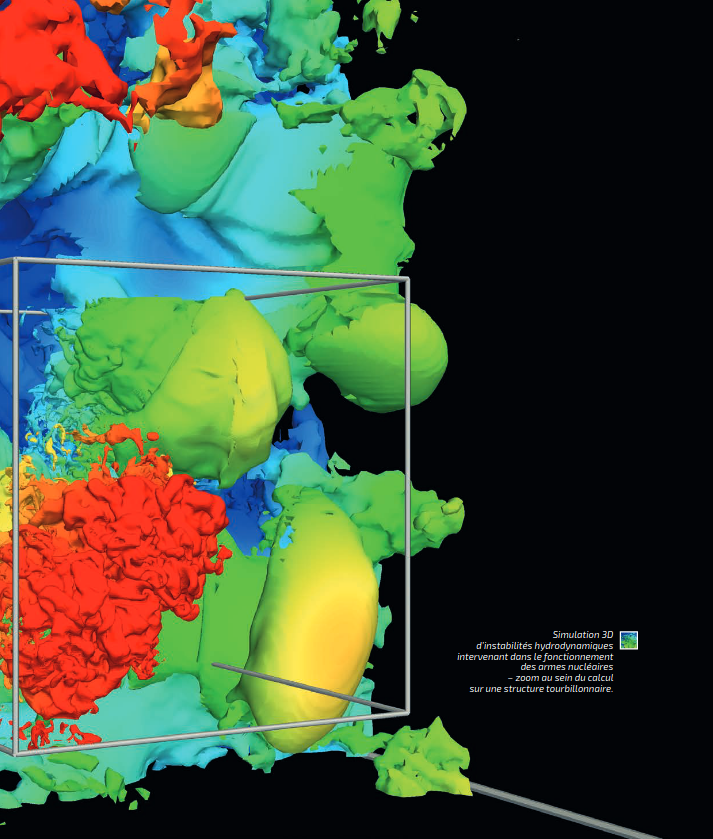
\includegraphics[height=5cm]{Assets/Physique_arme.png}
        %\caption{Liaisons entre les classes du moteur}
\end{figure}

\item \textbf{La simulation numérique} : reproduisant leur fonctionnement à l'aide de calculs et de modèles informatiques. Simuler une arme nuclaire nécessite d'un centaine à des centaines de millions de mailles ce qui implique que les systèmes d'équations associés ont alors des milliards d'inconnues. Cela nécessite alors de disposer d’ordinateurs très puissants
pour conserver une durée de calcul acceptable. Trois générations de supercalculateurs ont été définies et réalisées pour mettre en œuvre les standards de garantie : TERA 1, en 2001, avec 5 teraflops / TERA 10, en 2005, avec 50 teraflops /  TERA 100, en 2010, avec 1,3 petaflops

\begin{figure}[H]
    \hspace{0cm} % <<== Décale tout vers la gauche
    \begin{subfigure}[t]{0.42\textwidth}
        \centering
        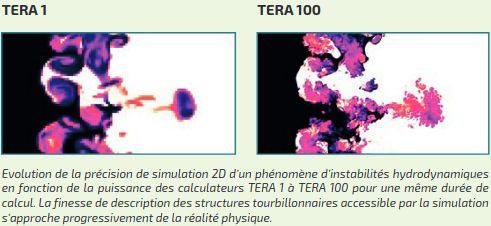
\includegraphics[height=5cm]{Assets/Exemple_Simulation.png}
        \caption{Liaisons entre les classes du moteur}
    \end{subfigure}
    \hspace{10em} % <<== Espace entre les deux images
    \begin{subfigure}[t]{0.42\textwidth}
        \centering
        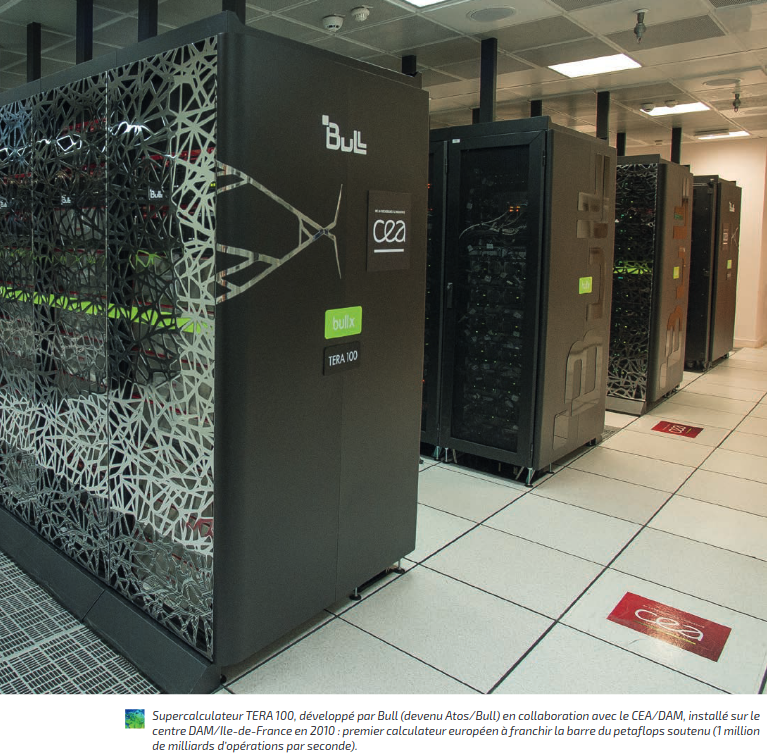
\includegraphics[height=5cm]{Assets/Supercalculateur.png}
        \caption{Supercalculateur utilisé pour les simulations}
    \end{subfigure}
    \caption{Illustrations du fonctionnement du programme Simulation}
    \label{fig:images}
\end{figure}

\item \textbf{La validation expérimentale} : vérifiant expérimentalement les résultats des simulations et des modélisations à l'aide de deux grandes installations, l'installation EPURE qui est une installation de radiographie dédiée à la phase non nucléaire du fonctionnement de l'arme et l'installation du Laser Mégajoule qui est un "laser de puissance" permettant de reproduire à toute petite échelle les conditions physiques dans lesquelles se trouve la matière lors du fonctionnement nucléaire de l'arme.
\end{itemize}

\section{Enjeux et objectifs}
... % à compléter



\chapter{Environnement technique}

Ce chapitre présente l'environnement numérique dans lequel j'ai évolué au CEA, les technologies que j'ai utilisées tout au long du stage ainsi que les contraintes associées à cet environnement.

\section{Technologies utilisées}
\section{Outils de développement}
\section{Contraintes techniques}
... % à compléter

\chapter{Veille technologique}
Ce que tu as appris ou approfondi pour comprendre les bases scientifiques ou techniques liées à l’outil/la machine/le principe physique utilisé dans ta mission.

Explications machine + phsique théorique sur les onde
Imagerie par Rayons X et par neutrons
... % à compléter
\section{Modélisation d'une chaîne radiographique}
\subsection{Présentation générale des techniques d'imagerie par rayonnements}
\subsubsection{Imagerie par rayons X}
L'imagerie par rayons X est la technique principale utilisée dans une chaîne radiographique. Les rayons X constituent une forme de rayonnement électromagnétique, au même titre que la lumière visible, l'ultraviolet, l'infrarouge, les micro-ondes, les ondes radio ou les rayons gamma.  
Une onde électromagnétique résulte de l'oscillation en phase d'un champ électrique et d'un champ magnétique perpendiculaires entre eux (voir figure~\ref{fig:...}). Elle se propage dans le vide à la vitesse de la lumière, soit \( c = 299\,792\,458 \, \text{m/s} \).  
Dans le cas d'une onde sinusoïdale ou monochromatique, la fréquence \(\nu\) et la période \(T\) sont reliées par \( T = 1/\nu \). La longueur d'onde \(\lambda\) correspond à la distance parcourue par l'onde en une période, soit \( \lambda = cT = c/\nu \).  
Les rayons X sont des ondes électromagnétiques dont les fréquences sont comprises entre \(10^{16}\) Hz et \(10^{20}\) Hz.

\begin{figure}[H]
    \centering
    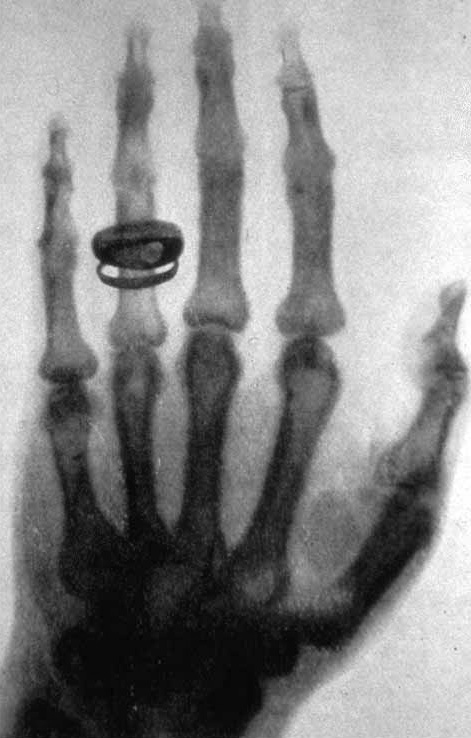
\includegraphics[height=5cm]{Assets/Exemple_xray.png}
    \caption{Exemple d'une image obtenue à partir de rayons X}
    \label{fig:images}
\end{figure}

\subsubsection{Imagerie neutronique}
L'imagerie neutronique repose sur les mêmes principes que l'imagerie par rayons X, mais les neutrons interagissent avec les noyaux des atomes plutôt qu'avec leurs électrons. Comme les rayons X, les neutrons sont atténués par certains éléments tels que l'hydrogène, le carbone, le bore ou le lithium, tout en étant capables de traverser de nombreux matériaux lourds. Cela confère à l'imagerie neutronique un avantage par rapport à l'imagerie par rayons X pour la visualisation en deux ou trois dimensions.En revanche, un inconvénient majeur de cette technique est qu'elle nécessite un flux élevé de neutrons pour obtenir des informations exploitables, ce qui impose l'utilisation de réacteurs nucléaires expérimentaux capables de produire un tel flux. Cette méthode est principalement utilisée dans l'industrie.

\begin{figure}[H]
    \centering
    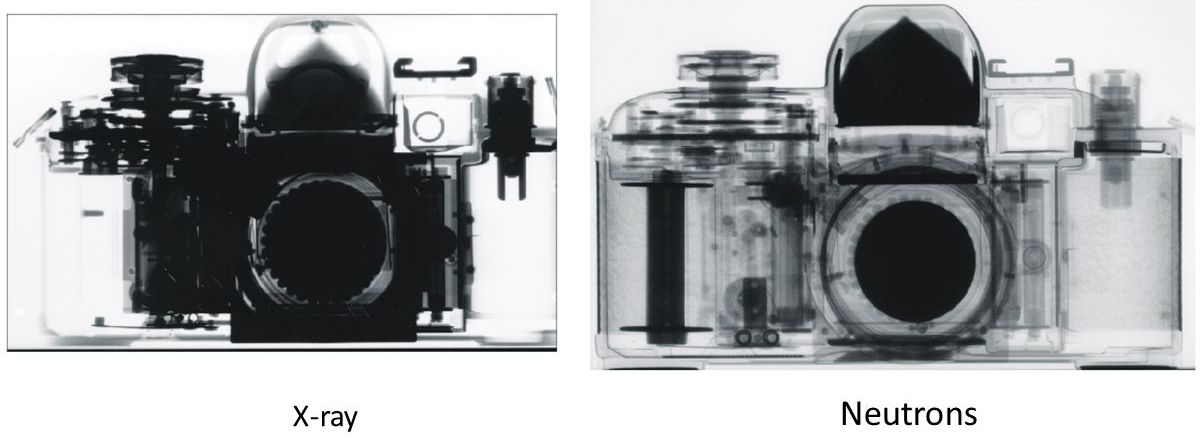
\includegraphics[height=5cm]{Assets/Imagerie_neutron_xray.png}
    \caption{Comparaison entre l'imagerie rayons X et l'imagerie neutronique}
    \label{fig:images}
\end{figure}

\subsection{Modélisation}
Les différentes méthodes d'imagerie ayant été exposées, il est maintenant important de comprendre comment fonctionne une chaîne radiographique de manière générale.

\paragraph{Production de rayons X}
\paragraph{Interactions rayons X / matière}
\paragraph{Détection}
\begin{itemize}
    \item Le processus de conversion des rayons X en signal électronique (ex : scintillateurs, photodiodes, détecteurs plans).
    \item Le modèle de réponse du détecteur (efficacité quantique, bruit de détection, résolution spatiale).
    \item L'influence des caractéristiques du détecteur sur la qualité de l'image finale (SNR, MTF).
\end{itemize}
\paragraph{Acquisition}
La phase d'acquisition regroupe le traitement du signal issu du détecteur pour former l'image numérique finale. Cette étape inclut :
\begin{itemize}
    \item La numérisation du signal (quantification, échantillonnage) ;
    \item L'application éventuelle de pré-traitements (correction du gain, réduction du bruit) ;
    \item Le formatage et l'optimisation des données pour l'affichage et l'analyse.
\end{itemize}

\section{Principe de fonctionnement de l'installation EPURE}
Le principe général d'une chaîne radiographique ayant été exposé, il est important de comprendre de manière plus précise comment fonctionne l'insatllaition EPURE.

\subsection{Description de l'installation}
\subsection{Les trois axes radiographiques}
\subsubsection{Le 1er axe radiographique : Airix}
\subsubsection{Le 2ème axe radiographique : Merlin}
\subsubsection{Le 3ème axe radiographique : Regrouper tous les sous parties en 1}
\subsection{Les trois axes radiographiques}
\subsection{Le déroulement d'une expérience à un axe radiographique}
\subsection{L'enregistrement d'images radiographiques}
\subsubsection{Gamma caméra}
\paragraph{Principe}
\paragraph{Détection}
\paragraph{Acquisition}


\chapter{Missions réalisées}
Présenter les principes que j'ai utilier ici --> description de toute la chaoine radiographique (--> desc de toutes les images, ce qu'elles représentent, ce qu'elles contiennent) + explications des prétraitements + mettre des profils d'image / histogrammes / métriques dans tableau / image, bref tout détailler  + expliquer la chronologie dans le détail


\section{Tâches effectuées}
\subsection{1ère tâche}
\subsection{2ème tâche}
\subsection{3ème tâche}
\subsection{Finalité}
\section{Méthodologie}
\section{Difficultés rencontrées}
... % contenu identique avec tâches, technos, outils, etc.
\subsection{Voir Gantt pour faire les autres sous chapitres}
\section{Améliorations possibles}



\chapter{Conclusion}

Cette conclusion clôture ce rapport en dressant un bilan du travail réalisé, en évoquant les pistes d'amélioration, et en ouvrant sur mes perspectives professionnelles.

\section{Bilan du stage}
physique + traitement d'images = C'est cool + faire un bilan global de ce qui a été fait + sur ce qui pourrait être fait

\section{Perspectives sur mon avenir}
% contenu identique
Ce stage m'a conforté dans mon souhait de poursuivre dans un domaine mêlant le traitement d'images et la physique. Je souhaite continuer à développer mes compétences dans cette double spécialité, en travaillant sur des projets alliant aspects théoriques et applications pratiques.  
Concernant la poursuite d'études, je me projette vers une éventuelle thèse, mais pas immédiatement. En effet, après trois années très intensives en Licence 3 et en Master, je préfère prendre une année pour approfondir mes choix, trouver un emploi afin de me reposer et identifier un sujet de doctorat qui corresponde pleinement à mes aspirations.

\chapter{Glossaire}



\appendix
\chapter{Annexes}

Cette section rassemble les éléments complémentaires et techniques relatifs au stage.

\chapter{Bibliographie}
% https://www.google.com/url?sa=t&source=web&rct=j&opi=89978449&url=https://reporterre.net/Bruyeres-le-Chatel-Essonne&ved=2ahUKEwjFm4m12vaMAxWufKQEHadBNEIQFnoECBMQAw&usg=AOvVaw3fVEsHbaAEx2_p7_cmjm5C
% https://www.cea.fr/presse/Documents/actualites/20-ans-programme-simulation.pdf
\end{document}
